\chapter{Signals}
\label{chapter_signals}

The signal definitions are stored in the OpenOffice document {\em Signals.ods}
for all plattforms.
As shown in fig. \ref{signals_ods} the perl script
{\em GenerateSignalDefinitions.pl} creates two files
{\em Signals.hh} and {\em Signals.hcc} containing the class definitions 
and static objects declarations. 

\begin{figure}[bpht]
\begin{center}
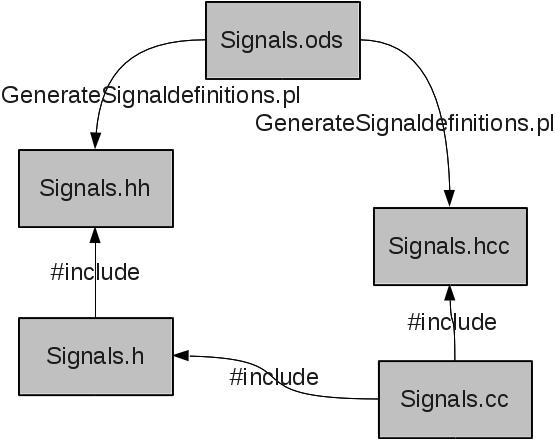
\includegraphics[width=10cm]{signals_ods.jpg}
\end{center}
\caption{Signal definitions by Spreadsheet}
\label{signals_ods}
\end{figure}

The generation is triggered by the plattform specific {\em Makefile}.
The script takes the desired target specifier(s) as command line
parameters.

\section{Signal Definition}
\label{sec_signal_definition}
The first sheet in {\em Signals.ods} contains the administrativ part.

\subsection{Grouping}
The signals are stored in groups. The definition of a group requires
an entry in the list of groups, which resides in the first sheet {\em GROUPS}
starting at line 3\footnote{This location must not be changed!}.
Each group entry consists of
\begin{description}
\item[Group name] which must have an identical name to the spreadsheet page.
   The sequence of spreadsheet pages must be identical to the sequence of
   group entries in this section.
\item[Group Number] defines the number region of the group.
    The {\em Group Number} is multiplied internally by 100.
    There may be 99 signals within each group.
\end{description}
The scripts checks for the matching of the group names and for multiple
usage of a group number.
The list of groups is terminated by an emtpy line.

\subsection{Groups}
Each group element contains the following entries:
\begin{description}
\item[GROUP INTERNAL ID] is the offset to the {\em Starting Number} of the 
   group. The id must be unique for all signals (not checked) to allow
   proper signal treatment by the runtime system.
   The {\em group internal id} 0 denotes the signal matching
   all signals defined in the group.
   The resulting signal {\em id} is created by the calculation of
   $GroupNumber \cdot 100 + GroupInternalId$
 
\item[ExceptionClass] defines the name of the C++ class, which shall be created.
   These names must by unique over all groups. This is also the name of
   the signal in the system part.
\item[ParentClass], which is used to build a C++ class hierarchy of the
    signals (C++ exceptions).
\item[System] specifies which plattform needs this signal. 
   The valid entries are defined by a drop down list. Please update the lists 
   on all sheets when a new plattform is added.
\item[Message] is the text which is sent to the standard output, when this
    signal was detected by the default signal handler.
\item[Description] contains the description of the reason for this signal
   for the external plattform signal manual. TeX syntax is allowed.
\end{description}

The scripts captures all entries of all group sheet with a matching
{\em System} entry.

\section{Decoration Scheme}
\begin{description}
\item[xxx] is the user supplied identifier for a signal
\item[\_xxx] is the (private) identifier with the concrete signal object
\item[generalized\_xxx] is the upcasted (public) identifier 
    of the concrete signal
\item[index\_xxx] is the enumeration item for the signal index within
   one procedure ore task

\item[lll] is the user defined identifer for a label 
\item[label\_lll] is the label in C++
\item[index\_lll] is the index of the label in the array for the computed goto

\end{description}

\section{Usage in System Part (is subject of change)}
A plattform specific signal is mapped to a user defined identifer in the 
system part. 

\begin{PEARLCode}
CHAR_OVERFLOW: CharacterTooLongSignal;
\end{PEARLCode}

\begin{CppCode}
static pearlrt::CharacterTooLongSignal _CHAR_OVERFLOW;
pearlrt::Signal * generalized_CHAR_OVERFLOW = &_CHAR_OVERFLOW;
\end{CppCode}

There is no possibility to define a signal upon its number, since this
produces lots of problems with the {\em static initialisation desaster}.
The identification of a signal at run time is done upon the signal id
which is referenced as {\em RST-value}.


\section{C++ Code for Signal Handler}
PEARL defines that a signal handler may be scheduled not inside 
a BEGIN/END-clause. The definition of a signal handler in a REPEAT block is also
prohibited. Thus we have access in the signal handler to all variables, which are defined
at the containing PROC or TASK level.
The definition of a signal handler inside of IF/THEN/ELSE-blocks is ok.

Possible reaction is a block of statements, which is executed and the
PROC is exited (the TASK teriminated) if the signal handler does not
contain a {\em GOTO-statement} defining the continuation point.

These code structure requires that only labels defined on task or proc level
may be used for this goto.

\begin{PEARLCode}
SYSTEM;
   overfl: FixedOverFlowSignal;    
   div0:   FixedDivideByZeroSignal;
   arith:  ArithmeticSignal;

 PROBLEM;
   SPC overfl SIGNAL;
   SPC div0   SIGNAL;
   SPC arith  SIGNAL;

   X: PROC (p FIXED) 
      DCL k FIXED(15);

      k := 2;

restart: 
      ! signal action #1
      ON overfl BEGIN
         PUT 'PROC X: Arithmetic error (returning)' TO console BY A, SKIP;
         RETURN;
      END;

      ! signal action #2
      IF ( p == 1) THEN
         ON overfl BEGIN
            PUT 'PROC X: Overflow occured (terminating)' TO console BY A, SKIP;
            TERMINATE;     
         END;
      FIN;
      
      IF ( p > 5) THEN
      ! signal action #3
        ON overfl BEGIN
           PUT 'PROC X: Overflow occured (returning)' TO console BY A, SKIP;
           RETURN;
        END;
      FIN;

      ! signal action #4
      ON div0 BEGIN 
          PUT 'Divide by zero (restarting)' TO console BY A, SKIP;
          IF ( p ==  6) THEN
             GOTO EXIT;
          FIN;
          IF ( p = 11) THEN
              k:= 11//(k-k);   ! produce new div0 which is not caught again
          FIN;
          p := 6;
          GOTO RESTART;
      END;
      
      IF p == 11 THEN
          k := 10 / (k-k);  ! force 'div by 0'
      FIN;

      FOR i TO 100 REPEAT
        k := k * k;
      END;
exit:
  END;
\end{PEARLCode}
There are four signal handler defined in the procedure.
Since there are signals handler defined in the procedure,
the body is placed in a try-catch-block.
The catch block checks, whether the current signal matches 
on of the scheduled signal actions.

\begin{CppCode}
// system part
static pearlrt::FixedRangeSignal _overfl;
pearlrt::Signal *generalized_overfl = &_overfl;


static pearlrt::FixedDivideByZeroSignal _div0;
pearlrt::Signal *generalized_div0 = &_div0;

static pearlrt::ArithmeticSignal _arith;
pearlrt::Signal *generalized_arith = &_arith;

extern pearlrt::Signal *generalized_overfl;
extern pearlrt::Signal *generalized_div0;
extern pearlrt::Signal *generalized_arith;

// problem part
SPCTASK(TASK1);

void _x(pearlrt::Task * me, pearlrt::Fixed<15> p) {
   pearlrt::Fixed<15> _k;

   //[ generated from ON statements in PROC
   static pearlrt::ScheduleSignalAction sigActions[] = {
		pearlrt::ScheduleSignalAction(generalized_arith),
		pearlrt::ScheduleSignalAction(generalized_overfl),
		pearlrt::ScheduleSignalAction(generalized_div0)};

   const size_t NBROFSIGACTIONS = 
		sizeof(sigActions)/sizeof(sigActions[0]);

   enum signalIndex{index_arith, index_overfl, index_div0};
   int indexOfSignalAction = -1; // no action -> execute proc body
   //]


      // local decls
      _k = pearlrt::Fixed<15>(2);

label_restart:  // user label

   //[ autogenerated due to ON statements in PROC 
   //    (after decls before first statement but after fisrt label)
tryAgain:    // << autogen
   try {
      switch(indexOfSignalAction) {
          case -1: break;
          //[ generated from signal action #1 in PROC
          case 1:
             sigActions[index_arith].disable();
             printf("proc x: arithmetic error (returning)\n");
             return; // if in PROC; else me->terminate(me);
             sigActions[index_arith].enable();
          //]
          //[ generated from signal action #2 in PROC
          case 2:
             sigActions[index_overfl].disable();
             printf("proc x: Overflow occured (terminating)\n");
             sigActions[index_overfl].enable();
             me->terminate(me);
          //]
          //[ generated from signal action #3 in PROC
          case 3: 		 // signal action #3
             sigActions[index_overfl].disable();
                printf("proc x: Overflow occured (returning)\n");
             sigActions[index_overfl].enable();
               return; // if in PROC; else me->terminate(me);
          //]
          //[ generated from signal action #4 in PROC
	  case 4:               // signal action #4
              // disable div0 for this handler
              sigActions[index_div0].disable();
                // code for PUT 'PROC X: divide by 0 (restarting)'
                // TO console BY A, SKIP;
              printf("proc x: divide by 0 (restarting)\n");
              if ((p == pearlrt::Fixed<15>(6)).getBoolean()) {
                 sigActions[index_div0].enable();
                 goto label_exit;                 
              } 
              if ((p == pearlrt::Fixed<15>(12)).getBoolean()) {
	         _k = pearlrt::Fixed<15>(11)/(_k-_k);
              } 
              
              p = pearlrt::Fixed<15>(6);
              sigActions[index_div0].enable();
              goto label_restart;                 
              
          //]
      } // end of switch
   //]

   printf("---  x(%d) ---------------\n",p.x);


      //[ generated from ON
      sigActions[index_arith].setActionIndex(1);
      //]
       
      if ((p == pearlrt::Fixed<15>(1)).getBoolean()) {
         //[ generated from ON
         sigActions[index_overfl].setActionIndex(2);
      //]
      }

      if ((p > pearlrt::Fixed<15>(5)).getBoolean()) {
         //[ generated from ON
         sigActions[index_overfl].setActionIndex(3);
         //]
      }
     
      //[ generated from ON
      sigActions[index_div0].setActionIndex(4);
      //]

      if ((p == pearlrt::Fixed<15>(11)).getBoolean()) {
         _k = pearlrt::Fixed<15>(10)/(_k-_k);
      }

      if ((p == pearlrt::Fixed<15>(12)).getBoolean()) {
         _k = pearlrt::Fixed<15>(10)/(_k-_k);
      }

      {
         pearlrt::Fixed<15> _i;    // loop counter is auto gen.
         for (_i = 1;
            (_i<=pearlrt::Fixed<15>(100)).getBoolean(); 
            _i = _i + pearlrt::Fixed<15>(1)) {
             _k =  _k * _k;
         }
      }
label_exit:    //<< user label
	/* nop */ ;
   //[ generated due to ON statements in PROC
   } catch (pearlrt::Signal & s) {
      indexOfSignalAction = pearlrt::ScheduleSignalAction::getAction(
		&s, NBROFSIGACTIONS, sigActions);
      printf("got exception: indexOfAction=%d\n", indexOfSignalAction);
      if (indexOfSignalAction == 0) {
        // no active handler found
        throw;
      }
      goto tryAgain;
   } // end of catch
   //] end of generated code
}
\end{CppCode}


Remarks:
\begin{description}
\item[disable signal handler] is done if the signal handler becomes
   active. The handler is enables at the end of the signal handlers
   statements. In detail, this is only necessray, if the handler is exited 
   with a GOTO statment --- even at intermediate GOT-statements in the handler.
\item[generated identifiers]  may use different decorations if
   suitable for the compiler.
\item[sigActions] must be of type auto to provide task specific 
   signal reactions.
\item[sigGoto] must be of type auto to provide task specific 
   signal reactions.
\item[labels] should be defined as static, for speedup reasons
\end{description}

\section{C++ Code for Signal Handler with RST-Tag}
When a RST-element is specified in the ON-statement, the current
RST-value must be read into the given variable.

\begin{PEARLCode}
DCL Errorcode FIXED(15);
...
   ! 2nd ON statement in proc/task
   ON overfl RST(Errorcode) ...
\end{PEARLCode}

Currently there is a problem with the headers of Signal and Fixed.
Therefore the type \verb|Fixed<x>| may not be used inside the Signal-class.
The statement {\em RST(Errorcode)} modifies the code in the signal handler
alternative towards.

\begin{CppCode}
Fixed<15> _Errorcode;
...
case 2:
   _Errorcode.x = s.getCurrentRst();
   ...
\end{CppCode}
Obviously the used variable in RST must be defined on module,
 task or procedure level. 

\section{Induce}
The statement {\em INDUCE} simulates a signal and causes the trigger 
of the scheduled reaction.
Induce may specify a RST-value, which causes to raising of the 
signal with the given number.
In this case a temporary RST-value is set inside the signal structure.
This does not affect the identification of the signal.


\begin{PEARLCode}
INDUCE div_0;
INDUCE div_0 RST (1234);
\end{PEARLCode}

\begin{CppCode}
generalized_div0->induce();
generalized_div0->induce(1234);
\end{CppCode}

\begin{PEARLCode}
SYSTEM;
   TaskRunningSignal: Signal(102);
   Arithmetic: Signal(200);

PROBLEM;
   SPC TaskRunningSignal SIGNAL;
   SPC Arithmetic SIGNAL;
   DCL Errorcode Fixed;
   DCL counter FIXED INIT(0);

Prog: TASK MAIN;
    ALL 1 SEC ACTIVATE Demo;
END;

Demo: TASK; 
   counter := counter + 1;

   ON TaskRunningSignal RST(ErrorCode)
	PUT 'TaskSignal occured with RST=', ErrorCode TO console BY A,F,SKIP;
   ON Arithimetic RST(ErrorCode)
	PUT 'Arithmetic problem occured with RST=', ErrorCode TO console BY A,F,SKIP;

   Test;
END;

Test: PROC;
   CASE counter
   ALT /* 1 */ INDUCE TaskRunningSignal RST(200);
   ALT /* 2 */ INDUCE TaskRunningSignal;
   ALT /* 3 */ INDUCE TaskRunningSignal RST(200);
   FIN;
END;
\end{PEARLCode}

This program will produce the output
\begin{verbatim}
TaskSignal occured with RST=200
TaskSignal occured with RST=102
TaskSignal occured with RST=200
\end{verbatim}
The setting of the RST-value to 102 (which is the error code of 
the {\em Arithmetic} does not affect the signal identification.
The setting of the RST-value is done with another version of the 
induce()-method, which allows an {\em int} value as parameter.

Since signals are global objects the feature of setting the RST at
induce should be used with care. The implementation is not safe against
race conditions.

Sample C++ code for procedure {\em Test}:
\begin{CppCode}
void _Test(pearlrt::Task * me) {
   switch(_counter.x) {
      case 1: 
       generalized_TaskRunningSignal->induce(200);
       break;
      case 2: 
       generalized_TaskRunningSignal->induce();
       break;
      case 3: 
       generalized_TaskRunningSignal->induce(200);'
       break;
    }
}
\end{CppCode}

